\appendix
\section{相关工作}
\label{appendix:related_work}

\subsection{大规模后训练中的OPD}



传统的知识蒸馏通常在教师生成的响应上训练学生模型，导致训练过程中观察到的序列与学生在推理时生成的序列之间存在不匹配。GKD通过获取教师对学生生成序列的反馈来减少这种不匹配~\cite{agarwal2024policy}。MiniLLM进一步将语言模型蒸馏形式化为反向KL最优化，并开发了一种同策略策略梯度估计量\cite{gu2024minillm}。最近，思维机器实验室提出了OPD，作为一种实用的后训练范式，结合了学生端的探索与稠密的token级教师监督~\cite{lu2025onpolicydistillation}。


OPD及其多教师变体随后成为大规模大模型后训练的重要组成部分。近期的技术报告利用它们来整合独立训练的领域专家，并将多种能力融合到单一模型中~\cite{
coreteam2026mimov2flashtechnicalreport,
xu2026deepseek,
yang2026nemotron,
huang2026kat,
team2026mach}。这些研究为OPD的实际有效性与可扩展性提供了有力证据。然而，它们主要评估最终集成模型的表现，而未系统地分离在训练和评估分布受控变化下，提炼出的能力是否具备泛化性~\citep{li2026rolereasoningpatternsgeneralization,ren2026rethinkinggeneralizationreasoningsft,chu2025sft,garcia2025exploringllmscapturerepresent}。

\subsection{理解OPD机制}


最近的研究探讨了OPD取得成功所需的条件。
\citet{li2026rethinking} 将兼容的教师-学生思维模式和真正新颖的教师能力识别为有效蒸馏的两个重要因素。


其他研究则关注OPD的最优化病态问题。
\citet{fu2026revisiting} 分析了采样 token 最优化中的偏差与方差，识别出学生生成前缀的不可靠指导以及分词器不匹配为主要失效模式。  
一项互补研究将 OPD 描述为一种探索机制，并强调学生-教师不匹配和长度利用是两种核心病理~\cite{wang2026demystifying}。


多种方法通过修改其展开或最优化过程来提升OPD性能。  
早停OPD将监督限制在较早的响应位置，从而降低教师指导受学生前缀漂移的影响 \cite{ziheng2026less}。  
非对称OPD对正向量和非正向量优势采用不同的最优化处理方式，以平衡利用与模仿 \cite{jia2026asymmetric}。  
尽管这些研究解释并缓解了局部训练失败问题，我们关注的是一个互补性问题：OPD是否能在难度、语言、推理范围、任务领域以及模型原点之间实现迁移。

\subsection{OPD中的数据选择}


数据选择在大语言模型推理的强化学习中得到了广泛研究~\cite{yu2026dapo,kong2026rethinking,li2025learnalign}。  
越来越多的工作通过选择或重新加权其监督信号来改进OPD。  
SCOPE将正确的学生轨迹与错误的学生轨迹分离，强调教师对错误回放轨迹的纠正置信度以及学生对正确轨迹的不确定性~\cite{zheng2026scope}。  
FiRe-OPD首先过滤不可靠的轨迹，然后对保留轨迹中的信息性token进行软重加权~\cite{li2026filter}。  
BRTS采样多个教师轨迹，并根据教师的正确性以及与当前学生的对齐程度来选择监督信号~\cite{zhang2026policy}。  
Uni-OPD通过双视角策略，联合考虑学生侧的探索和教师侧的监督可靠性~\cite{hou2026uni}。


这些方法在不同粒度上选择监督信号，但并未直接决定是否应过滤教师未解决的查询，或保留学生已掌握的查询。我们通过受控的教师端过滤和学生端动态采样，将这两个因子分离，并进一步比较它们在不同模型原点情景下的影响。

\subsection{MOPD中的能力交互}


多教师同策略蒸馏（MOPD）通过将学生生成的轨迹路由至对应的教师，实现对单个学生的逐 token 监督~\cite{ma2026mopd}。在集成前独立训练领域专家，MOPD 降低了异构强化学习目标之间的直接耦合，并提供了一种可扩展的能力集成方法。


然而，来自多个教师的监督可能并不相互兼容。CaMOPD识别出由冲突的教师梯度引起的恢复—保持对抗效应，以及由于对具有不同修正需求的样本进行均匀组合而导致的弱信号平坦化现象\cite{chen2026counteraction}。它通过解耦最优化和基于教师-学生差距的样本选择来解决这些问题。


我们的工作从互补的跨领域泛化视角研究能力交互。我们不仅将每个教师视为仅传递其名义上的专长技能，还考察其更广泛的能力特征如何传递到主要领域和非主要领域。

\section{实验情景}
\label{sec:appendix_exp_setting}

\subsection{数据集}
\label{sec:appendix_datasets}

\subsubsection{训练数据集}
\label{sec:appendix_training_datasets}

\paragraph{数学推理}

我们使用 Big-Math-RL-Verified~\cite{albalak2025big} 作为主要的数学训练语料库。  
在绝对难度对比中，可用的 GSM8K~\cite{cobbe2021traininggsm8k} 和 DeepMath-103K-Hardest~\cite{he2026deepmathk} 语料库各自包含约 8K 个查询。  
因此，我们从 Big-Math-RL-Verified 中采样一个匹配的 8K 查询子集，以确保对比结果不受唯一训练查询数量的影响。

\paragraph{代码推理。}

我们使用 DeepCoder-Preview-Dataset~\cite{deepcoder2025} 进行代码领域 OPD。该数据集包含约 24K 个编程竞赛题目，每个题目都配有可执行的测试用例。其训练集包括从 2023 年 5 月 1 日到 2024 年 7 月 31 日期间提交的 LiveCodeBench~\cite{jain2025livecodebench} 题目，以及来自 TACO~\cite{li2023taco} 和 PrimeIntellect 的 SYNTHETIC-1~\cite{2025synthetic1} 的已验证题目。

\paragraph{科学推理。}

在单教师跨领域实验中，我们使用TextbookReasoning~\cite{fan2025megascience}作为科学领域的训练语料库。我们移除了所有标注为数学或计算机科学的样本，以减少与数学和代码领域的直接重叠。在MOPD实验中，我们遵循Nemotron-Research-Reasoning-Qwen-1.5B~\cite{liu2026prorl}训练所用的数据领域。科学数据来自SCP-116K~\cite{lu2025scp}，在过滤掉所有归类为数学的样本后获得。


\paragraph{指令执行。}

MOPD 中使用的指令遵循数据来自 Llama-Nemotron-后训练数据集~\cite{bercovich2025llamanemotron} 的 RL/指令遵循划分。我们将这些示例与筛选后的 SCP-116K 数据一起，构建科学/指令遵循训练池。科学和指令遵循示例各占科学/指令遵循池的 $50\%$。

\subsubsection{评估基准}
\label{sec:appendix_evaluation_datasets}

\paragraph{英语数学推理}

英语数学得分是 AMC~2023~\cite{MAA_AMC}、MATH-500~\cite{hendrycks2021measuringmath500}、AIME~2025/2026~\cite{MAA_AIME}、BeyondAIME~\cite{bytedance_seed_2025_beyondaime} 以及 OlymMATH-Hard~\cite{sun2026olymmath} 得分的平均值。

\paragraph{中国数学推理。}

中文数学得分是 OlymMATH-ZH~\cite{sun2026olymmath} 和 LiveMathBench-ZH~\cite{liu2025livemathbench} 的平均得分。

\paragraph{长期推理的数学问题。}

长期预测数学得分是 R-HORIZON~\cite{lu2025r} 中 AIME24-Horizon-2 和 AMC23-Horizon-4 的平均得分。

\paragraph{代码推理。}

我们在 2024 年 8 月 1 日至 2025 年 2 月 1 日期间发布的 LiveCodeBench v5 问题上评估代码生成能力~\cite{jain2025livecodebench}，采用 DeepCoder 所使用的评估方法。


\paragraph{科学与指令遵循。}

我们在 GPQA-Diamond~\cite{rein2023gpqa} 上评估科学推理能力，在 IFEval~\cite{zhou2023instructionfollowingevaluationlargelanguage} 上评估指令遵循能力。  
GPQA-Diamond 包含物理学、化学和生物学领域的专家级问题，而 IFEval 用于评估对可程序验证指令的遵守情况。



\subsection{模型}
\label{sec:appendix_models}

\subsubsection{模型谱系}
\label{sec:appendix_model_lineage}

我们使用模型谱系来区分同源和跨源OPD之间的差异。具体而言，当两个模型共享相同的实际初始化检查点，并且其中一个或两个模型都是从该检查点进一步进行后训练得到时，这两个模型被视为同源。

根据此定义，DeepSeek-R1-Distill-Qwen-1.5B~\cite{guo2025deepseekr1} 构成一个谱系根节点。  
JustRL-DeepSeek-1.5B~\cite{he2025justrl} 是通过对该检查点应用面向数学的强化学习后训练得到的，而  
Nemotron-Research-Reasoning-Qwen-1.5B~\cite{liu2026prorl} 则是通过从相同初始化状态进行长时间多领域强化学习获得的。  
Dev-1.5B 也从 DeepSeek-R1-Distill-Qwen-1.5B 初始化，并通过 10 步科学/IF OPD 进一步训练。  
因此，这四个模型属于同一谱系。  
DeepSeek-R1-Distill-Qwen-7B 与 Polaris-7B~\cite{Polaris2025} 构成第二个谱系，因为 Polaris-7B 是对 7B 版本的蒸馏检查点进一步后训练所得。  
同样地，DeepSeek-R1-Distill-Qwen-14B 与 Light-R1-14B~\cite{wen2025lightr1} 构成第三个谱系。  
对于 Qwen3 模型，Qwen3-4B~\cite{yang2025qwen3} 与 Polaris-4B 属于同一谱系，因为 Polaris-4B 是从 Qwen3-4B 后训练而来。  
Qwen3-8B 与 Qwen3-32B 被视为独立的谱系根节点，因为二者之间不存在彼此通过后训练获得的关系。

\begin{table*}[t]
    \centering
    \small
    \caption{
    我们实验中所用模型的后训练谱系。  
共享相同谱系根的模型被视为同源。
    }
    \label{tab:model_lineage}
    \resizebox{\linewidth}{!}{
    \begin{tabular}{llll}
        \toprule
        \textbf{Model} &
        \textbf{Lineage Root} &
        \textbf{Post-Training from the Root} &
        \textbf{Experimental Role} \\
        \midrule

        DS-R1-Distill-Qwen-1.5B
        & DS-R1-Distill-Qwen-1.5B
        & None
        & Student \\

        JustRL-DeepSeek-1.5B
        & DS-R1-Distill-Qwen-1.5B
        & Math-oriented RL
        & Teacher \\

        Nemotron-Research-Reasoning-Qwen-1.5B
        & DS-R1-Distill-Qwen-1.5B
        & Multi-domain prolonged RL
        & Teacher \\

        Dev-1.5B
        & DS-R1-Distill-Qwen-1.5B
        & 10-step science/IF OPD
        & Student \\

        \midrule

        DS-R1-Distill-Qwen-7B
        & DS-R1-Distill-Qwen-7B
        & None
        & Student \\

        Polaris-7B
        & DS-R1-Distill-Qwen-7B
        & Math-oriented RL
        & Teacher \\

        \midrule

        DS-R1-Distill-Qwen-14B
        & DS-R1-Distill-Qwen-14B
        & None
        & Student \\

        Light-R1-14B
        & DS-R1-Distill-Qwen-14B
        & Long-CoT reasoning RL
        & Teacher \\

        \midrule

        Qwen3-4B
        & Qwen3-4B
        & None
        & Student \\

        Polaris-4B
        & Qwen3-4B
        & Math-oriented RL
        & Teacher \\

        \midrule

        Qwen3-8B-SFT
        & Qwen3-8B
        & SFT on OpenThoughts3-1.2M
        & Student \\

        \midrule

        Qwen3-32B
        & Qwen3-32B
        & None
        & Teacher \\

        \bottomrule
    \end{tabular}
    }
\end{table*}

\subsection{训练配置}
\label{sec:training_config}

大多数配置在 100--200 步内收敛，因此我们将最大步数设置为 200。  
提示词批量大小为 128，每轮运行最多可使用 $200\times128=25.6$ K 个提示词实例。  
对于每个提示词，学生模型生成四个独立的同策略响应，对应于轨迹组大小为 $N=4$。  
标准的轨迹解码参数为：温度 $1.0$，top-$p$  $1.0$，以及无限制的 top-$k$ 采样，实现方式为 top-$k=-1$。

最大序列长度取决于教师-学生配置，如表~\ref{tab:max_sequence_length} 所总结。

\begin{table*}[t]
    \centering
    \caption{用于OPD推出和评估的最大序列长度。}
    \label{tab:max_sequence_length}
    \resizebox{0.8\linewidth}{!}{
    \begin{tabular}{lc}
        \toprule
        \textbf{Model Group} &
        \textbf{Maximum Length} \\
        \midrule

        Qwen3-4B, Qwen3-8B, Qwen3-32B, Polaris-4B
        & 40K \\

        DS-distill-1.5B,
        JustRL-1.5B, Nemotron-1.5B
        & 96K \\

        Light-R1-14B, DS-distill-14B
        & 64K \\

        Polaris-7B, DS-distill-7B 
        & 96K \\

        \bottomrule
    \end{tabular}
    }
\end{table*}



\subsection{评估配置}


在基准评估中，我们使用温度 $1.0$ ，top-$p$  $0.95$ ，
以及 top-$k=-1$ 。  
最大序列长度遵循
表~\ref{tab:max_sequence_length}。  
对于每个查询，我们独立采样 $K$ 个响应，并报告
$\operatorname{Avg@}K$ ，定义为

\begingroup
\begin{align*}
    \operatorname{Avg@}K
    =
    \frac{1}{|\mathcal{D}|}
    \sum_{x\in\mathcal{D}}
    \frac{1}{K}
    \sum_{k=1}^{K}
    \mathcal{V}\!\left(x,y^{(k)}\right),
    \label{eq:avg_at_k}
\end{align*}
\endgroup

其中 $y^{(k)}$  是第 $k$ 个独立采样的响应，  
$\mathcal{V}$  是特定于基准的验证器。  
与 Pass@$K$ 不同，Avg@$K$ 独立评估每个采样响应，  
并且不从 $K$ 次生成中选择最佳响应。

每个基准所使用的评估样本数量汇总于表~\ref{tab:evaluation_sampling_num} 中。

\begin{table}[t]
    \centering
    \caption{
    用于基准评估的独立采样响应数量。
    }
    \label{tab:evaluation_sampling_num}
    \resizebox{0.3\columnwidth}{!}{
    \begin{tabular}{lc}
        \toprule
        \textbf{Benchmark} & \textbf{Metric} \\
        \midrule

        AMC 2023
        & Avg@16 \\

        MATH-500
        & Avg@1 \\

        AIME 2025
        & Avg@16 \\

        AIME 2026
        & Avg@16 \\

        BeyondAIME
        & Avg@5 \\

        OlymMATH-Hard
        & Avg@5 \\

        OlymMATH-Easy
        & Avg@5 \\

        OlymMATH-ZH
        & Avg@5 \\

        R-HORIZON
        & Avg@10 \\

        LiveMathBench-ZH
        & Avg@16 \\

        GPQA-Diamond
        & Avg@4 \\

        LiveCodeBench v5
        & Avg@10 \\

        IFEval
        & Avg@4 \\

        \bottomrule
    \end{tabular}
    }
\end{table}


仅用于可视化，我们使用中心移动平均对评估曲线进行平滑处理。
令 $\{s_t\}$ 表示原始评估序列，
$\widetilde{s}_t$ 表示显示的值。
我们计算

\begingroup
\begin{align*}
    \widetilde{s}_t
    =
    \begin{cases}
        s_1,
        & t=1, \\[2pt]
        \displaystyle
        \frac{1}{3}\sum_{j=1}^{3}s_j,
        & t=2, \\[8pt]
        \displaystyle
        \frac{1}{5}\sum_{j=t-2}^{t+2}s_j,
        & t\geq 3.
    \end{cases}
\end{align*}
\endgroup

因此，第一个显示的点未进行平滑处理，第二个点对前一个、当前和后一个检查点进行平均，后续所有点均使用半径为二的五点中心移动平均。
原始训练轨迹在图中所示最终步数之外仍有延伸，因此从第三个点开始，所有显示的点均可获得完整的五点窗口，包括靠近右侧边界处的点。
中心移动平均常用于抑制局部波动，同时保留序列的主要趋势\citep{hyndman2018forecasting}。
平滑仅用于可视化，不影响任何报告的表格数值、检查点选择或统计计算。

\subsubsection{答案提取指令}
对于所有数学和科学推理基准，我们添加系统提示，并从每个模型的响应中提取最终 \texttt{\textbackslash boxed\{\}} 表达式内的答案，然后使用 Math-Verify\footnote{\url{https://github.com/huggingface/Math-Verify}} 用于解析和比较提取的答案与参考答案的库。  
对于数学任务，我们提示模型将最终答案（通常是数字和数学表达式，有时是选项）放在 \texttt{\textbackslash boxed\{\}} 内。  
\begin{insightbox}  
\textbf{数学推理任务（MATH-500, AMC23, AIME25/26, BeyondAIME, ...）：}\\  
请逐步推理，并将最终答案放入 \texttt{\textbackslash boxed\{\}} 中。  
\end{insightbox}  
对于 GPQA-Diamond，我们提示模型将最终选项（A、B、C 或 D）放入 \texttt{\textbackslash boxed\{\}}。  
\begin{insightbox}  
\textbf{科学推理任务（GPQA-Diamond）：}\\  
请逐步推理，并将最终答案（仅选项，即 A、B、C 或 D）放入 \texttt{\textbackslash boxed\{\}} 中。  
\end{insightbox}  
注意，上述两个系统提示与本文所用的所有模型保持一致。




\section{额外的实验结果}
\label{sec:appendix_add_results}
\subsection{训练数据难度的额外结果}

为了进一步检验所观察到的行为是否在仅基于单一数据集构建的难度划分之外依然成立，我们引入了两个额外的数据集，代表难度谱的两极。对于极端困难的情景，我们使用 DeepMath-103K~\cite{he2026deepmathk}，该数据集提供从 1 到 9 的难度得分，并保留得分高于 8 的查询。对于极端简单的情景，我们使用 GSM8K 训练集，该数据集包含小学数学应用题。我们在这两个数据集上重复相同的 OPD 实验，以检验当训练查询几乎总是可解或几乎从不可解时，教师端通过率是否变得更加重要。

图~\ref{fig:extreme_difficulty} 展示了实验结果。在两种难度极端情况下的实验得出了相似的结论。无论是小学水平的 GSM8K 查询还是极具挑战性的 DeepMath-103K 查询，通过 OPD 均获得了显著提升，且在所有测试配置下，它们的最终平均得分差异不足两分。因此，有效的同策略监督并不要求训练查询处于狭窄的绝对难度值域内。然而，在任一难度极端上训练的模型，通常仍落后于在更具多样性的 Big-Math-RL-Verified 混合数据集上训练的模型。这表明，尽管教师通过率或绝对查询难度本身并不能单独决定一个样本是否有效，但保持对问题难度的广泛覆盖，对于实现更广泛的泛化能力仍然有益。


\begin{figure*}[t]
    \centering
    \begin{subfigure}[b]{0.32\linewidth}
        \centering
        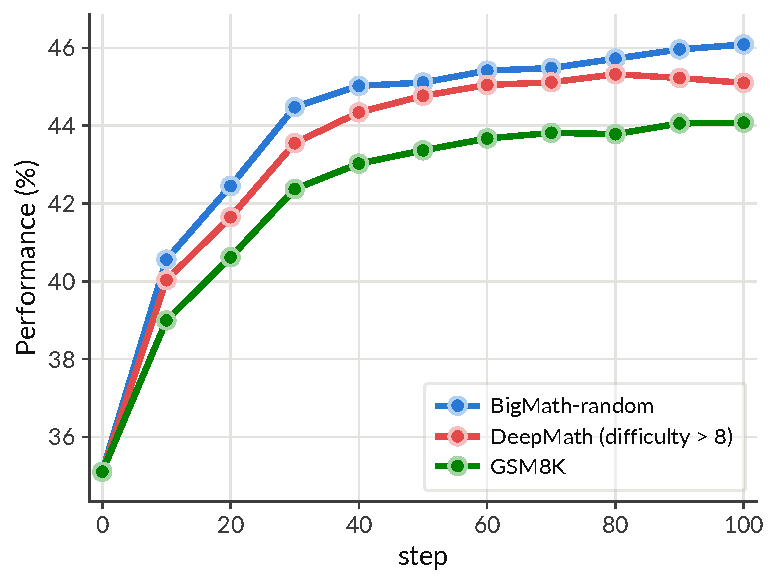
\includegraphics[width=\linewidth]{latex/figures/findings_1/teacher_pass_rate/1d5b_to_1d5b_math_teacher_difficulty_mainmath6_avg.pdf}
        \caption{JustRL-1.5B $\rightarrow$ DS-distill-1.5B}
        \label{fig:difficulty_1d5b_to_1d5b}
    \end{subfigure}
    \hfill
    \begin{subfigure}[b]{0.32\linewidth}
        \centering
        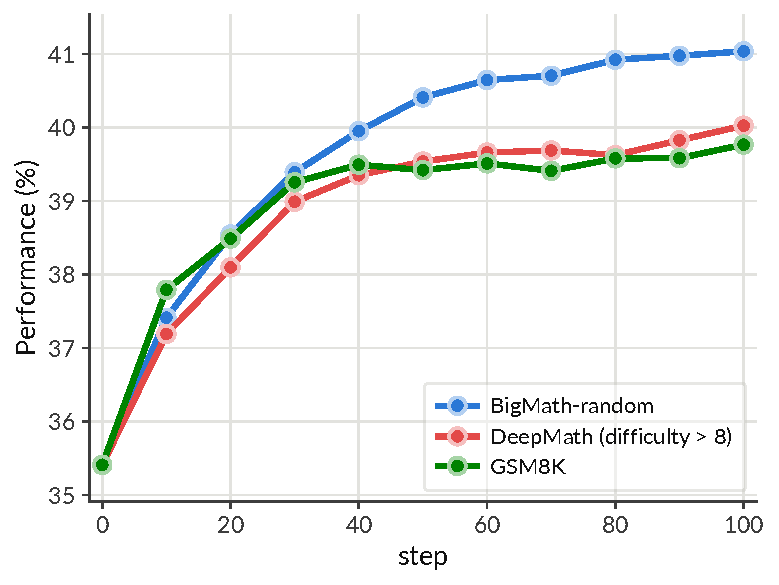
\includegraphics[width=\linewidth]{latex/figures/findings_1/teacher_pass_rate/7b_to_1d5b_math_teacher_difficulty_mainmath6_avg.pdf}
        \caption{Polaris-7B $\rightarrow$ DS-distill-1.5B}
        \label{fig:difficulty_7b_to_1d5b}
    \end{subfigure}
    \hfill
    \begin{subfigure}[b]{0.32\linewidth}
        \centering
        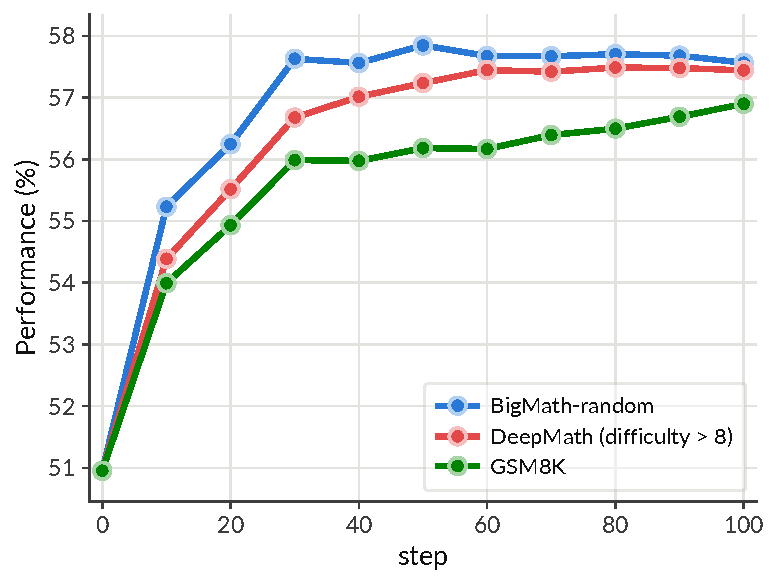
\includegraphics[width=\linewidth]{latex/figures/findings_1/teacher_pass_rate/7b_to_7b_math_teacher_difficulty_mainmath6_avg.pdf}
        \caption{Polaris-7B $\rightarrow$ DS-distill-7B}
        \label{fig:difficulty_7b_to_7b}
    \end{subfigure}

    \caption{领域内数学性能（六个英文基准的平均值）对训练查询的难度变化不敏感。子图（a--c）分别在极简单的GSM8K、极困难的DeepMath-103K以及多样化的BigMath混合数据集上进行训练。}
    \label{fig:extreme_difficulty}
\end{figure*}

\subsection{模型原点的额外泛化结果}
\label{sec:appendix_additional_generalization}


图~\ref{fig:math_generalization_and_code_generalization} 展示了在三种教师-学生配置下的额外泛化结果。每个面板报告了在英文数学、中文数学、长时序数学和代码任务上的性能，使我们能够共同考察领域内分布变化和跨领域迁移。

图~\ref{fig:4b_to_4b} 展示了同源的 Polaris-4B $\rightarrow$ Qwen3-4B 配置。  
我们对比了在随机采样的 Big-Math-RL-Verified 子集上的 OPD 与在 Polaris-53K（Polaris-4B 后训练所用数据集）上的 OPD。  
两种训练分布均产生稳定的性能提升，并在评估基准上收敛至相似水平。  
该结果表明，有效的 OPD 并不需要访问教师模型原始的后训练数据。  
图~\ref{fig:32b_to_8b} 报告了跨源的 Qwen3-32B $\rightarrow$ Qwen3-8B-SFT 配置，其在 Big-Math-RL-Verified 上进行训练。  
Qwen3-8B-SFT 从 Qwen3-8B-Base 初始化，并在 OPD 前基于 OpenThoughts3-1.2M 进行监督微调。  
学生模型在英文数学、中文数学以及长时序数学任务上均有明显提升，表明数学监督能够有效跨越语言和推理时序的变化实现迁移。  
相比之下，代码性能仅发生微小变化。  
该结果说明，在跨源师生配置下，广泛领域的泛化能力并不必然意味着对每个语义领域都具有同等强度的迁移效果。  
图~\ref{fig:14b_to_14b} 展示了同源的 Light-R1-14B $\rightarrow$ DS-distill-14B 配置。  
OPD 在所有四个评估组中均带来稳定提升。  
尤为值得注意的是，在长时序数学任务上，蒸馏后的学生模型最终以显著优势超越独立教师模型。  
这一观察表明，最终的学生模型并不必然受限于教师模型独立基准下的准确率。

\subsection{完整的跨领域迁移结果}
\label{sec:appendix_complete_others_to_math}

图~\ref{fig:cross_domain_generalization_others_to_math} 展示了从代码和科学训练数据迁移到数学推理的完整结果。第一行展示了 DS-distill-1.5B 的结果，第二行则展示了 DS-distill-7B 的对应结果。对于每个学生模型，我们评估了英文数学、中文数学以及长时序数学问题的表现。在两种模型大小下，使用代码或科学查询的 OPD 通常能提升数学推理能力，尽管这些实验中并未使用任何数学查询。这种提升不仅体现在标准英文基准上，还扩展到了中文问题和组合型长时序问题。这证实了教师的数学能力可以通过从非数学领域收集的学生轨迹实现迁移。

完整的曲线进一步证实了主文中报告的模型-原点效应。同源教师在三个评估分布上通常产生更强且更稳定的提升。在同一教师谱系内，数学、代码和科学监督实验之间的差异相对较小，而改变教师原点则会产生更大的性能差距。因此，教师-学生后训练关系对跨领域迁移的影响，可能比训练查询的名义领域更具影响力。

我们进一步考察了指令遵循数据是否可以作为数学能力迁移的载体。图~\ref{fig:if_to_math_cross_domain_generalization} 报告了 Nemotron-1.5B $\rightarrow$ DS-distill-1.5B 以及 Polaris-7B $\rightarrow$ DS-distill-7B 的结果。两种配置均在英文数学、中文数学上进行了评估。即使学生轨迹是从指令遵循提示中收集的，教师仍然能够传递那些未在名义训练领域中明确表示的能力。结合之前的结果，这表明训练查询主要决定了教师监督的触发位置，而非严格限制哪些教师能力可以被迁移。

\subsection{MOPD 的完整数学结果}
\label{sec:appendix_mopd_full_math}

表~\ref{tab:mopd_math_full_result} 报告了 MOPD 实验在训练步数 200 时的完整数学推理结果。  
在第一种教师–领域分配方案下，JustRL 提供数学监督，Nemotron 提供科学/IF 监督。  
以 JustRL 为主导的混合方案通常保持更强的数学性能。  
$25/8$ 配置实现了最高的平均得分 $19.6\%$，略高于仅使用 JustRL 的配置以及均衡的 $1/1$ 混合方案。  
此外，一旦 Nemotron 成为主导，数学性能便显著下降：  
平均得分从均衡混合方案的 $19.1\%$ 下降至 $17.4\%$（对应 $2/25$）以及 Nemotron 单独配置的 $14.9\%$。  
该关系在各个基准上并非严格单调，但总体趋势表明，过多的 Nemotron 监督会使学生偏向 Nemotron 较弱的数学能力。

反向分配提供了互补的证据。在此情景中，Nemotron 监督数学查询，而 JustRL 监督科学/IF 查询。尽管进行了这种重新分配，增加 JustRL 监督的比例仍能提升学生在数学任务上的表现。仅使用 JustRL 的配置平均得分为 $17.5\%$，而平衡配置和仅使用 Nemotron 的配置分别为 $15.8\%$。这一结果无法通过名义上的训练领域分配来解释，因为在该情景下，JustRL 并不监督数学数据。相反，其更强的数学能力是通过科学/IF 轨迹实现迁移的。因此，完整的基准测试结果证实，领域路由并不会将教师的影响限制在其指定的领域内。


\begin{figure*}[t]
    \centering

    \begin{subfigure}[b]{0.99\linewidth}
        \centering
        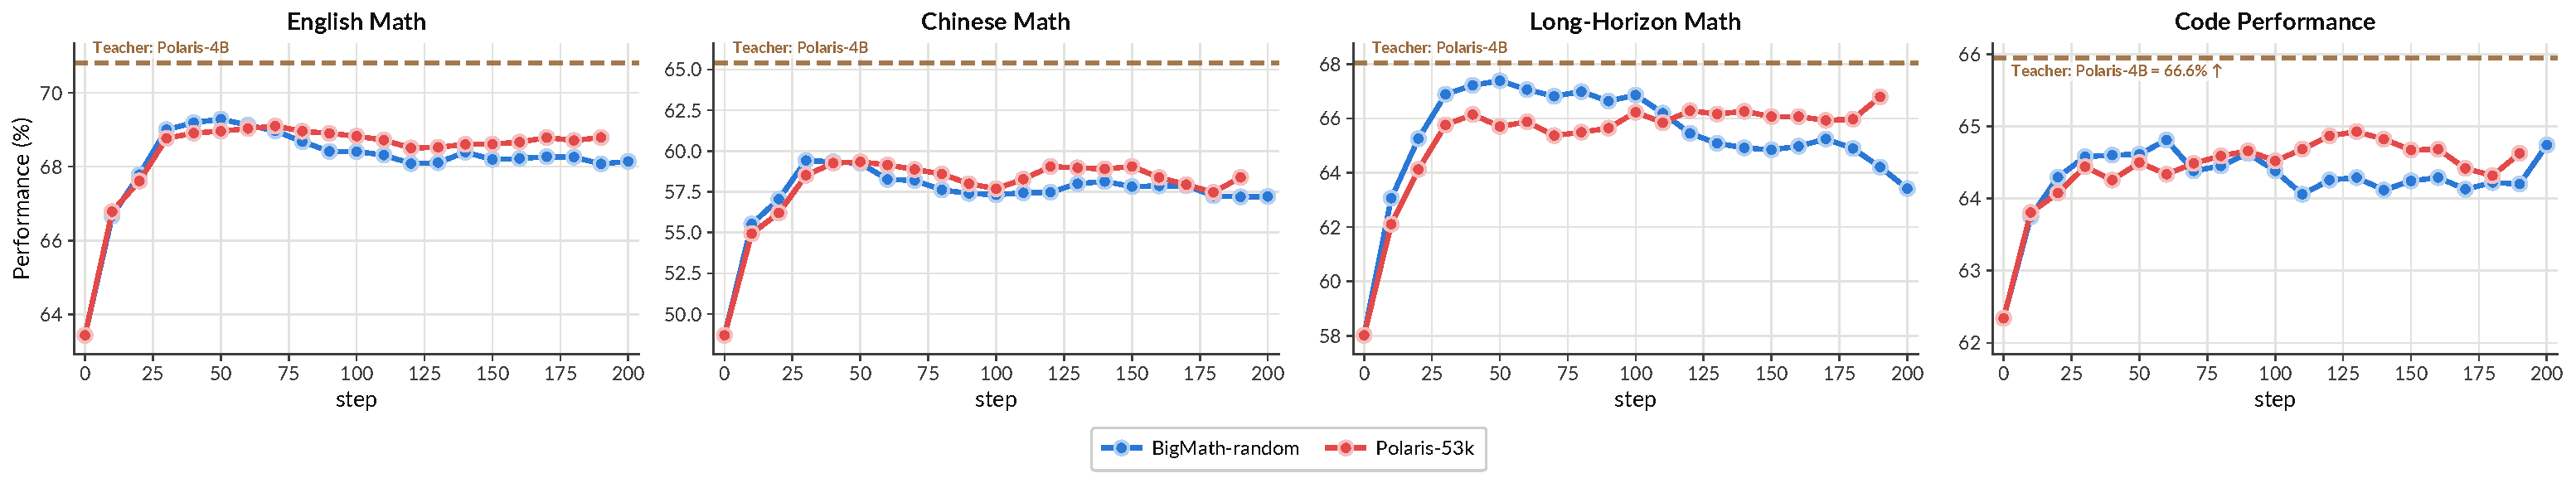
\includegraphics[width=\linewidth]{latex/figures/appendix/4b_polaris4b_qwen3_generalization_math_panel.pdf}
        \caption{Polaris-4B 到 Qwen3-4B}
        \label{fig:4b_to_4b}
    \end{subfigure}

    \begin{subfigure}[b]{0.99\linewidth}
        \centering
        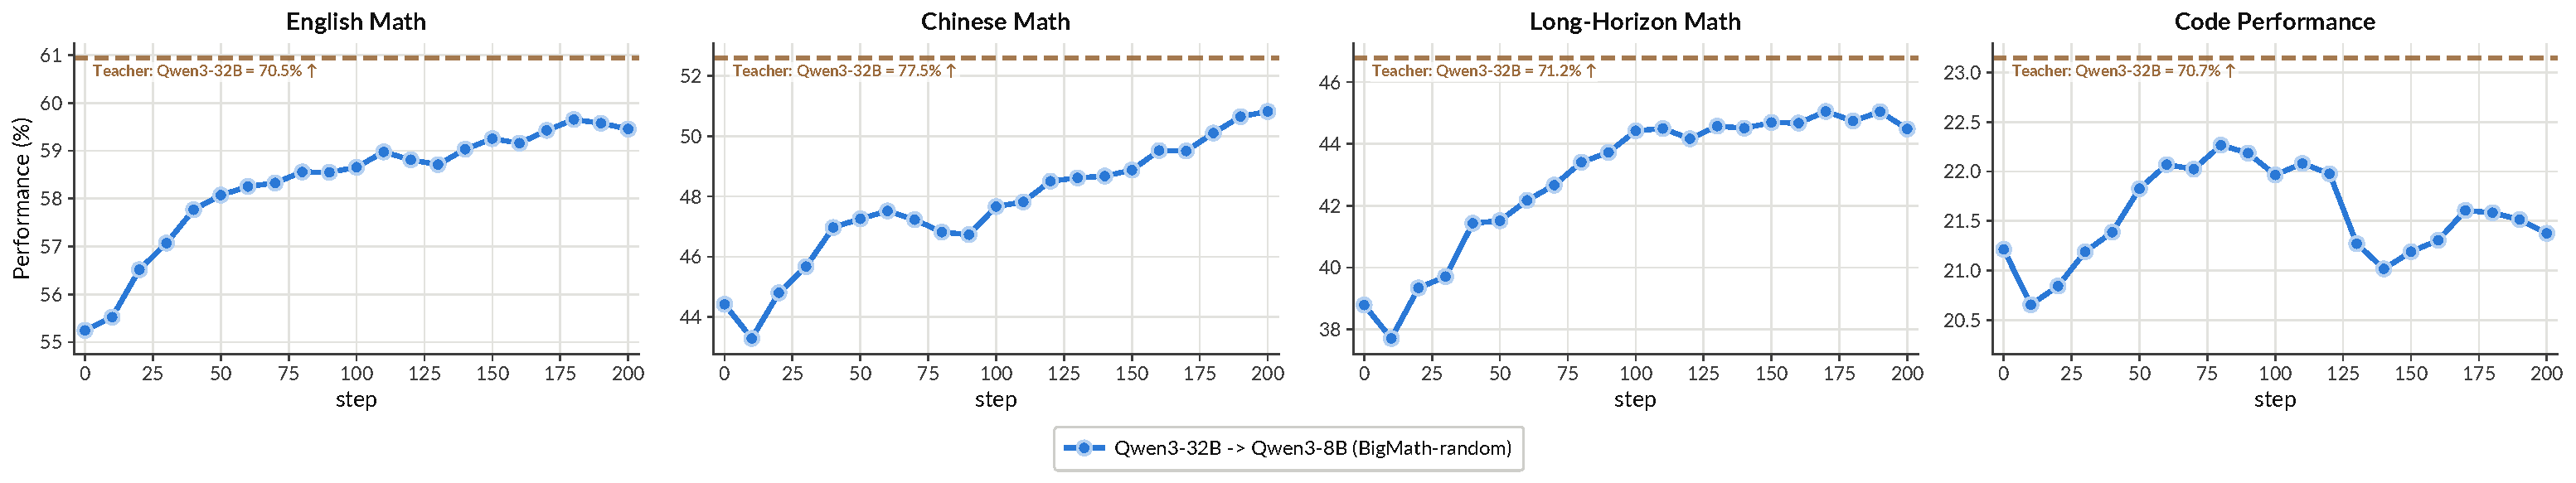
\includegraphics[width=\linewidth]{latex/figures/appendix/8b_qwen32b_bigmath_generalization_math_panel.pdf}
        \caption{Qwen3-32B 到 Qwen3-8B-SFT}
        \label{fig:32b_to_8b}
    \end{subfigure}

     \begin{subfigure}[b]{0.99\linewidth}
        \centering
        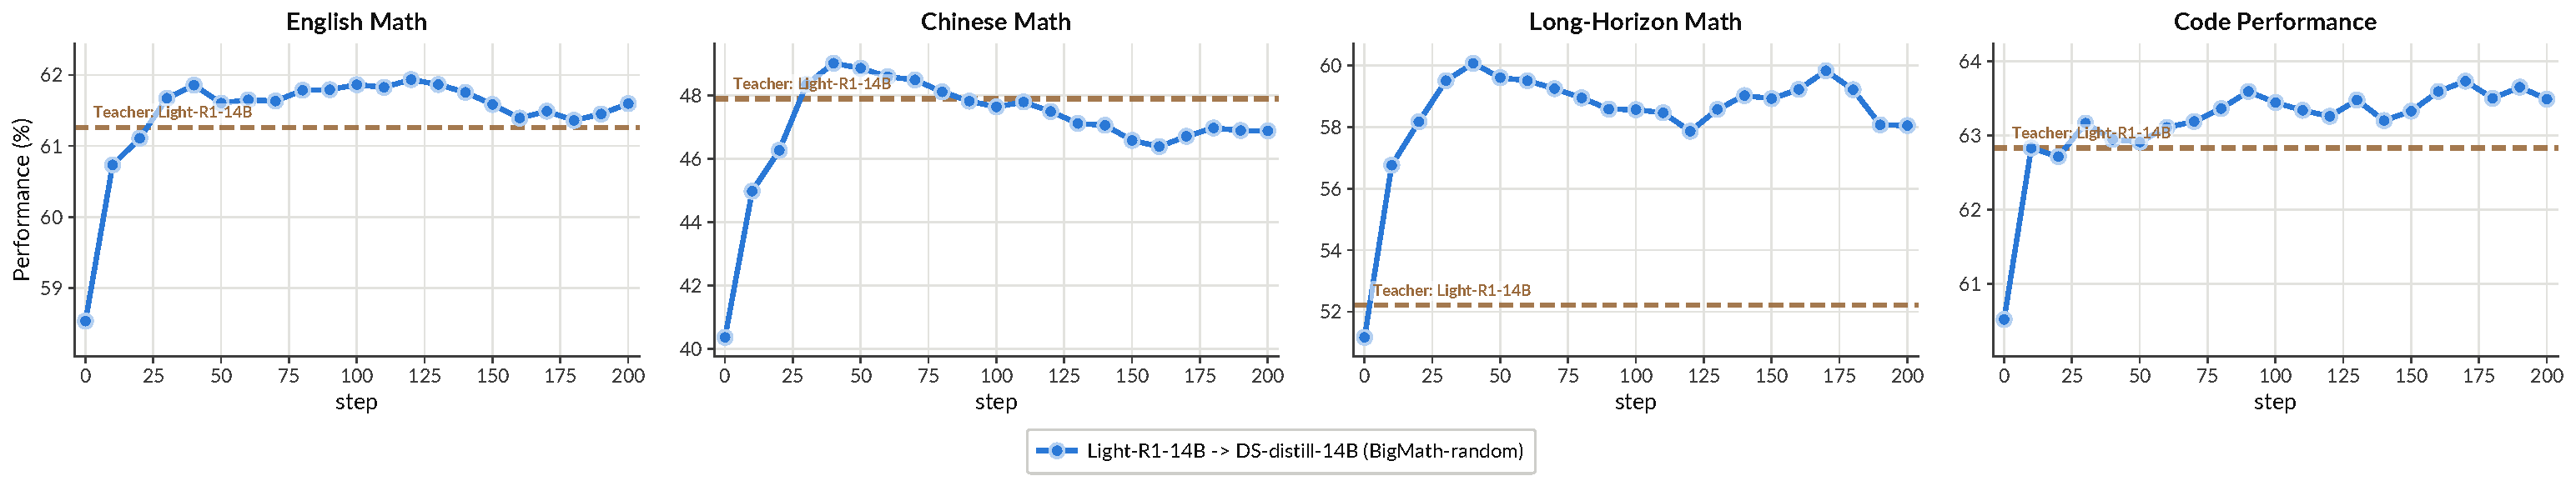
\includegraphics[width=\linewidth]{latex/figures/appendix/14b_lightr1_bigmath_generalization_math_panel.pdf}
        \caption{Light-R1-14B 到 DS-distill-14B}
        \label{fig:14b_to_14b}
    \end{subfigure}

    \caption{在三种教师-学生配置下的额外泛化结果。}
    \label{fig:math_generalization_and_code_generalization}
\end{figure*}

\begin{figure*}[t]
    \centering
    \captionsetup[subfigure]{font=scriptsize}
    \begin{subfigure}[b]{0.32\linewidth}
        \centering
        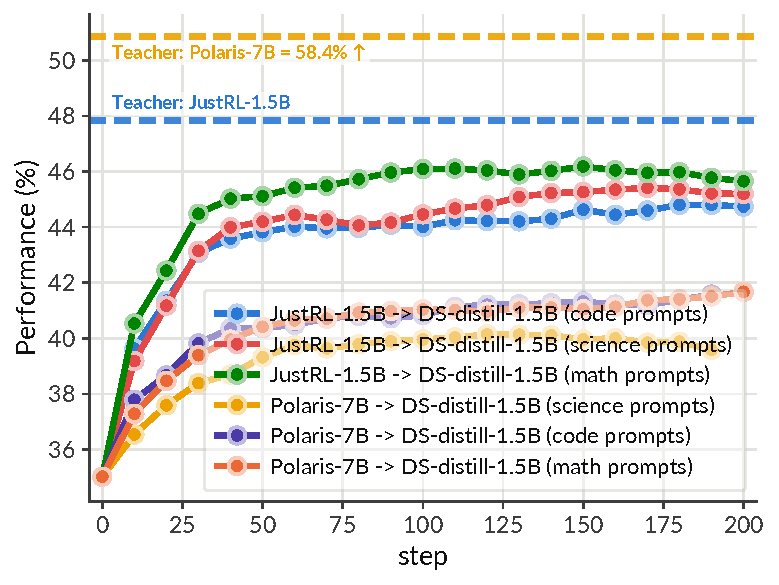
\includegraphics[width=\linewidth]{latex/figures/findings_2/1d5b_cross_domain_generalization_others_to_math_mainmath6_avg.pdf}
        \caption{数学（DS-distill-1.5B）}
        \label{fig:others_to_math_en_1d5b}
    \end{subfigure}
    \hfill
    \begin{subfigure}[b]{0.32\linewidth}
        \centering
        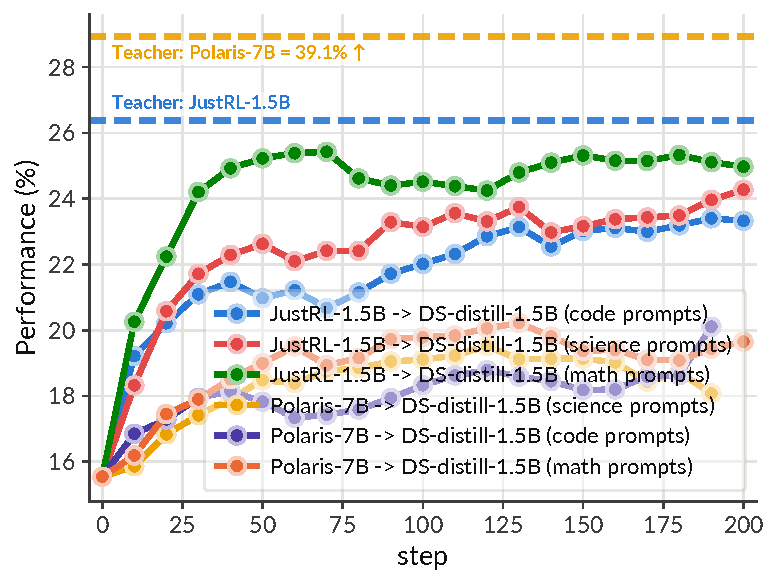
\includegraphics[width=\linewidth]{latex/figures/findings_2/1d5b_cross_domain_generalization_others_to_math_zh_avg.pdf}
        \caption{中国数学（DS-distill-1.5B）}
        \label{fig:others_to_math_zh_1d5b}
    \end{subfigure}
    \hfill
    \begin{subfigure}[b]{0.32\linewidth}
        \centering
        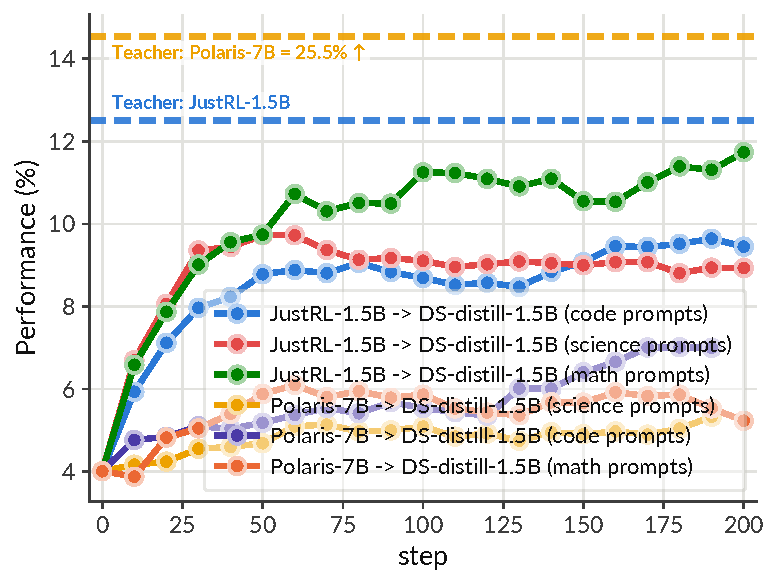
\includegraphics[width=\linewidth]{latex/figures/findings_2/1d5b_cross_domain_generalization_others_to_math_horizon_avg.pdf}
        \caption{长时程数学（DS-distill-1.5B）}
        \label{fig:others_to_math_horizon_1d5b}
    \end{subfigure}

     \begin{subfigure}[b]{0.32\linewidth}
        \centering
        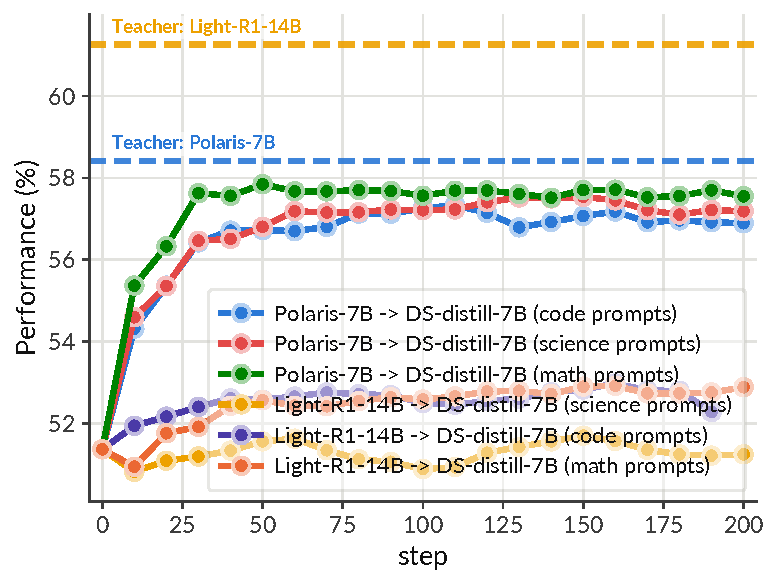
\includegraphics[width=\linewidth]{latex/figures/findings_2/7b_cross_domain_generalization_others_to_math_mainmath6_avg.pdf}
        \caption{数学（DS-distill-7B）}
        \label{fig:others_to_math_en_7b}
    \end{subfigure}
    \hfill
    \begin{subfigure}[b]{0.32\linewidth}
        \centering
        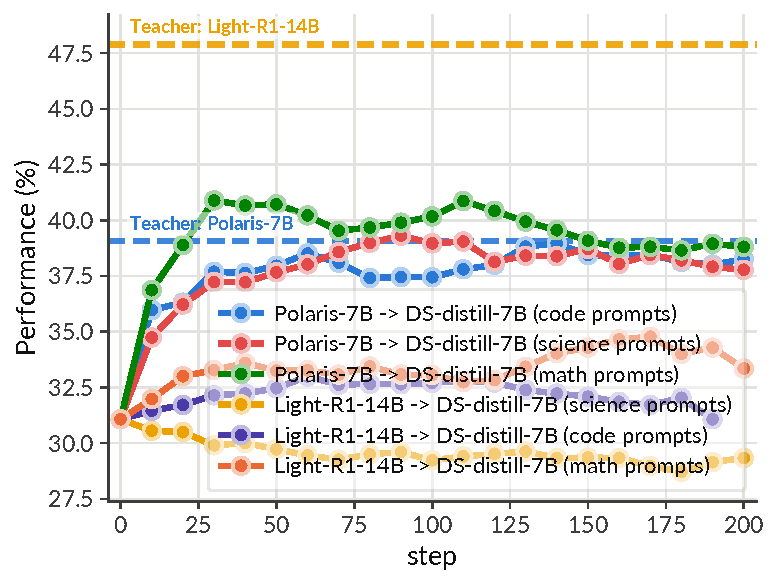
\includegraphics[width=\linewidth]{latex/figures/findings_2/7b_cross_domain_generalization_others_to_math_zh_avg.pdf}
        \caption{中文数学（DS-distill-7B）}
        \label{fig:others_to_math_zh_7b}
    \end{subfigure}
    \hfill
    \begin{subfigure}[b]{0.32\linewidth}
        \centering
        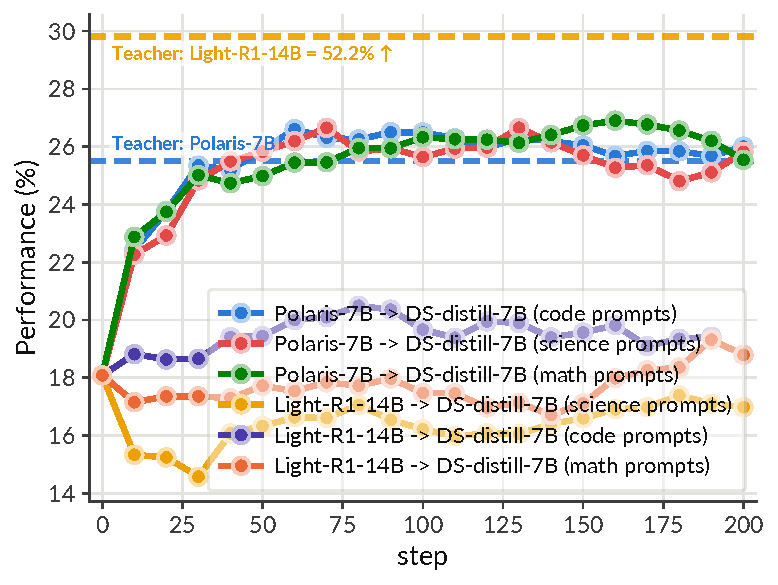
\includegraphics[width=\linewidth]{latex/figures/findings_2/7b_cross_domain_generalization_others_to_math_horizon_avg.pdf}
        \caption{长时程数学（DS-distill-7B）}
        \label{fig:others_to_math_horizon_7b}
    \end{subfigure}

    \caption{在代码和科学领域进行训练，并泛化到与数学相关的领域。}
    \label{fig:cross_domain_generalization_others_to_math}
\end{figure*}


\begin{figure*}[t]
    \centering
    \begin{subfigure}[b]{0.99\linewidth}
        \centering
        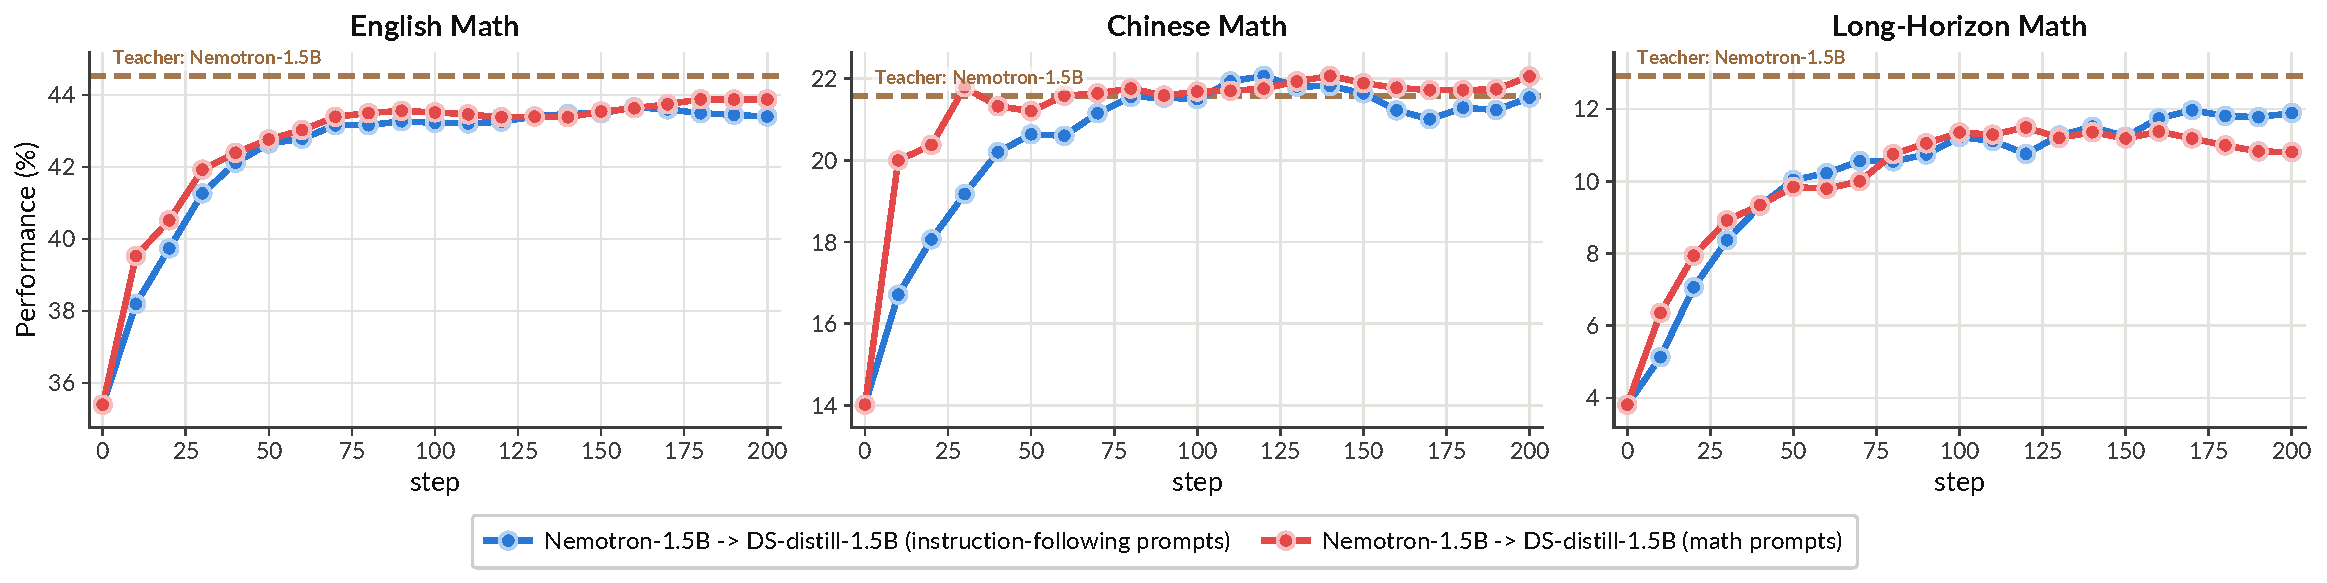
\includegraphics[width=\linewidth]{latex/figures/appendix/1d5b_nemo_if_to_math_generalization_math_panel.pdf}
        \caption{Nemotron-1.5B 到 DS-distill-1.5B}
        \label{fig:if_to_math_1d5b}
    \end{subfigure}

     \begin{subfigure}[b]{0.99\linewidth}
        \centering
        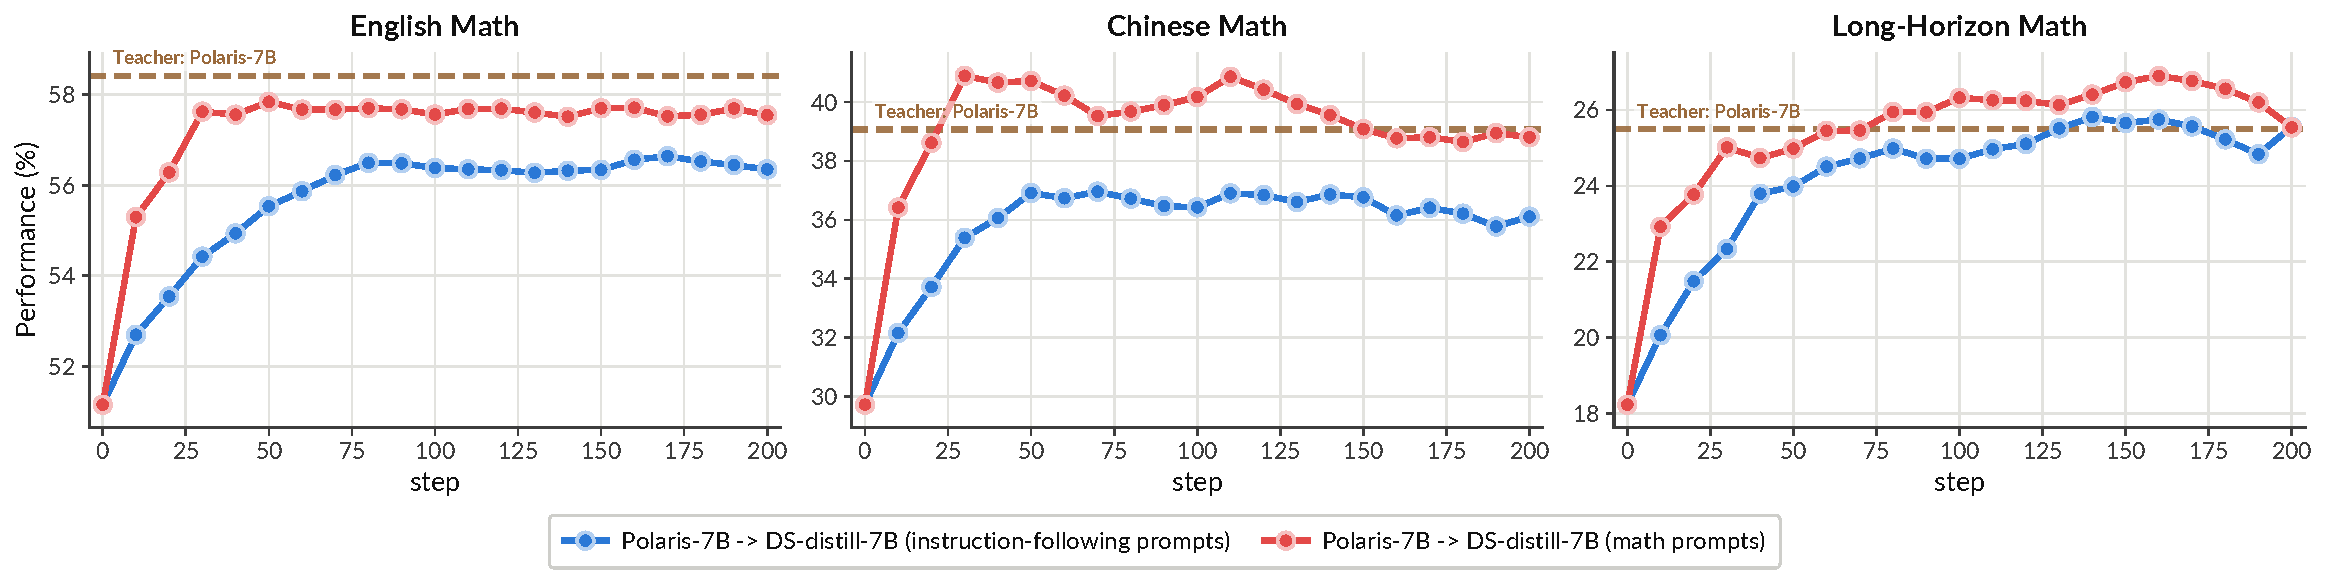
\includegraphics[width=\linewidth]{latex/figures/appendix/7b_polaris_if_to_math_generalization_math_panel.pdf}
        \caption{北斗七B至DS提炼七B}
        \label{fig:if_to_math_7b}
    \end{subfigure}

    \caption{在指令遵循数据上进行训练，并在数学相关基准上实现泛化。}
    \label{fig:if_to_math_cross_domain_generalization}
\end{figure*}

\begin{table*}[htbp]
\centering
\caption{MOPD 在五个数学推理基准上的性能比较（训练步数为200）。}
\label{tab:mopd_math_full_result}
\resizebox{\textwidth}{!}{%
\begin{tabular}{c|ccccc|c}
\toprule
\textbf{Configuration} & \textbf{BeyondAIME} & \textbf{OlymMATH-e(en)} & \textbf{OlymMATH-e(zh)} & \textbf{OlymMATH-h} & \textbf{AIME24-n2} & \textbf{Average} \\
\midrule
\midrule
DS-distill-1.5B & $9.6\%$ & $14.2\%$ & $11.2\%$ & $3.2\%$ & $6.0\%$ & $8.8\%$ \\
JustRL-1.5B & $19.0\%$ & $32.6\%$ & $23.0\%$ & $5.7\%$ & $16.3\%$ & $19.3\%$ \\
Nemotron-1.5B & $17.6\%$ & $29.2\%$ & $16.6\%$ & $5.6\%$ & $14.3\%$ & $16.7\%$ \\
\midrule
\midrule
\multicolumn{7}{c}{\textbf{\textit{Math Teacher: JustRL-1.5B, science/IF Teacher: Nemotron-1.5B, Student: DS-distill-1.5B}}} \\
\midrule

$\mathbf{\text{JustRL}/\text{Nemotron}=25/0}$ & $19.0\%$ & $32.6\%$ & $23.0\%$ & $5.7\%$ & $16.3\%$ & $19.3\%${\footnotesize \textcolor{green!60!black}{(\textbf{+0.2 pp})}} \\
$\mathbf{\text{JustRL}/\text{Nemotron}=25/2}$ & $19.4\%$ & $33.3\%$ & $23.0\%$ & $5.9\%$ & $14.1\%$ & $19.1\%${\footnotesize \textcolor{gray!60!black}{(\textbf{+0.0 pp})}} \\
$\mathbf{\text{JustRL}/\text{Nemotron}=25/8}$ & $19.6\%$ & $34.5\%$ & $23.2\%$ & $5.5\%$ & $15.3\%$ & $19.6\%${\footnotesize \textcolor{green!60!black}{(\textbf{+0.5 pp})}} \\
$\mathbf{\text{JustRL}/\text{Nemotron}=1/1}$ & $20.2\%$ & $32.4\%$ & $20.6\%$ & $5.0\%$ & $17.3\%$ & $19.1\%${\footnotesize \textcolor{black!60!black}{(\textbf{baseline})}} \\
$\mathbf{\text{JustRL}/\text{Nemotron}=8/25}$ & $19.7\%$ & $32.5\%$ & $22.7\%$ & $5.5\%$ & $15.7\%$ & $19.2\%${\footnotesize \textcolor{green!60!black}{(\textbf{+0.1 pp})}} \\
$\mathbf{\text{JustRL}/\text{Nemotron}=2/25}$ & $19.2\%$ & $31.0\%$ & $19.2\%$ & $5.2\%$ & $12.3\%$ & $17.4\%${\footnotesize \textcolor{red!60!black}{(\textbf{-1.7 pp})}} \\
$\mathbf{\text{JustRL}/\text{Nemotron}=0/25}$ & $15.9\%$ & $25.3\%$ & $15.7\%$ & $3.7\%$ & $13.8\%$ & $14.9\%${\footnotesize \textcolor{red!60!black}{(\textbf{-4.2 pp})}} \\

\midrule
\midrule
\multicolumn{7}{c}{\textbf{\textit{Math Teacher: Nemotron-1.5B, science/IF Teacher: JustRL-1.5B, Student: DS-distill-1.5B}}} \\
\midrule

$\mathbf{\text{JustRL}/\text{Nemotron}=25/0}$ & $18.2\%$ & $29.8\%$ & $21.1\%$ & $5.8\%$ & $12.3\%$ & $17.5\%${\footnotesize \textcolor{green!60!black}{(\textbf{+1.7 pp})}} \\
$\mathbf{\text{JustRL}/\text{Nemotron}=25/8}$ & $17.4\%$ & $28.0\%$ & $17.8\%$ & $4.5\%$ & $14.8\%$ & $16.5\%${\footnotesize \textcolor{green!60!black}{(\textbf{+0.7 pp})}} \\
$\mathbf{\text{JustRL}/\text{Nemotron}=1/1}$ & $17.3\%$ & $26.6\%$ & $16.8\%$ & $4.4\%$ & $13.9\%$ & $15.8\%${\footnotesize \textcolor{black!60!black}{(\textbf{baseline})}} \\
$\mathbf{\text{JustRL}/\text{Nemotron}=8/25}$  & $17.1\%$ & $26.2\%$ & $16.8\%$ & $4.7\%$ & $14.3\%$ & $15.8\%${\footnotesize \textcolor{gray!60!black}{(\textbf{-0.0 pp})}} \\
$\mathbf{\text{JustRL}/\text{Nemotron}=0/25}$ & $17.4\%$ & $26.5\%$ & $17.0\%$ & $4.5\%$ & $13.6\%$ & $15.8\%${\footnotesize \textcolor{gray!60!black}{(\textbf{-0.0 pp})}} \\
\bottomrule
\end{tabular}%
}
\end{table*}